
\documentclass[norsk,a4paper,12pt]{article}
\usepackage[T1]{fontenc} %for å bruke æøå
\usepackage[utf8]{inputenc}
\usepackage{graphicx} %for å inkludere grafikk
\usepackage{verbatim} %for å inkludere filer med tegn LaTeX ikke liker
\usepackage{mathpazo}
\usepackage{amsmath}
\bibliographystyle{plain}


\title{FYS 2140 Hjemmeeksamen}
\author{15053}
\date{\today}
\begin{document}

\maketitle



\section*{Oppgave 1}

\subsection*{a1)}

\begin{equation}
\lambda_C = \frac{h}{m_ec}
\end{equation}


\begin{align*}
\lambda_C &= comptonbølgelengden \\
h &= planckkonstanten \\
m_e &= elektronmassen \\
c &= lyshastighetetn \\
\end{align*}

Forskjellen i bølgelengde gis ved 

\begin{align*}
\Delta \lambda = (\lambda' - \lambda_0) = \frac{h}{m_ec}(1-cos\theta)
\end{align*}

\begin{equation}
\Delta\lambda = \lambda_C(1-cos\theta)
\label{eq:1}
\end{equation}


\begin{equation}
\lambda_C = \frac{h}{m_ec}= \underline{\underline{2.43 x 10^{-3} nm}}
\end{equation}





\begin{figure}[h]
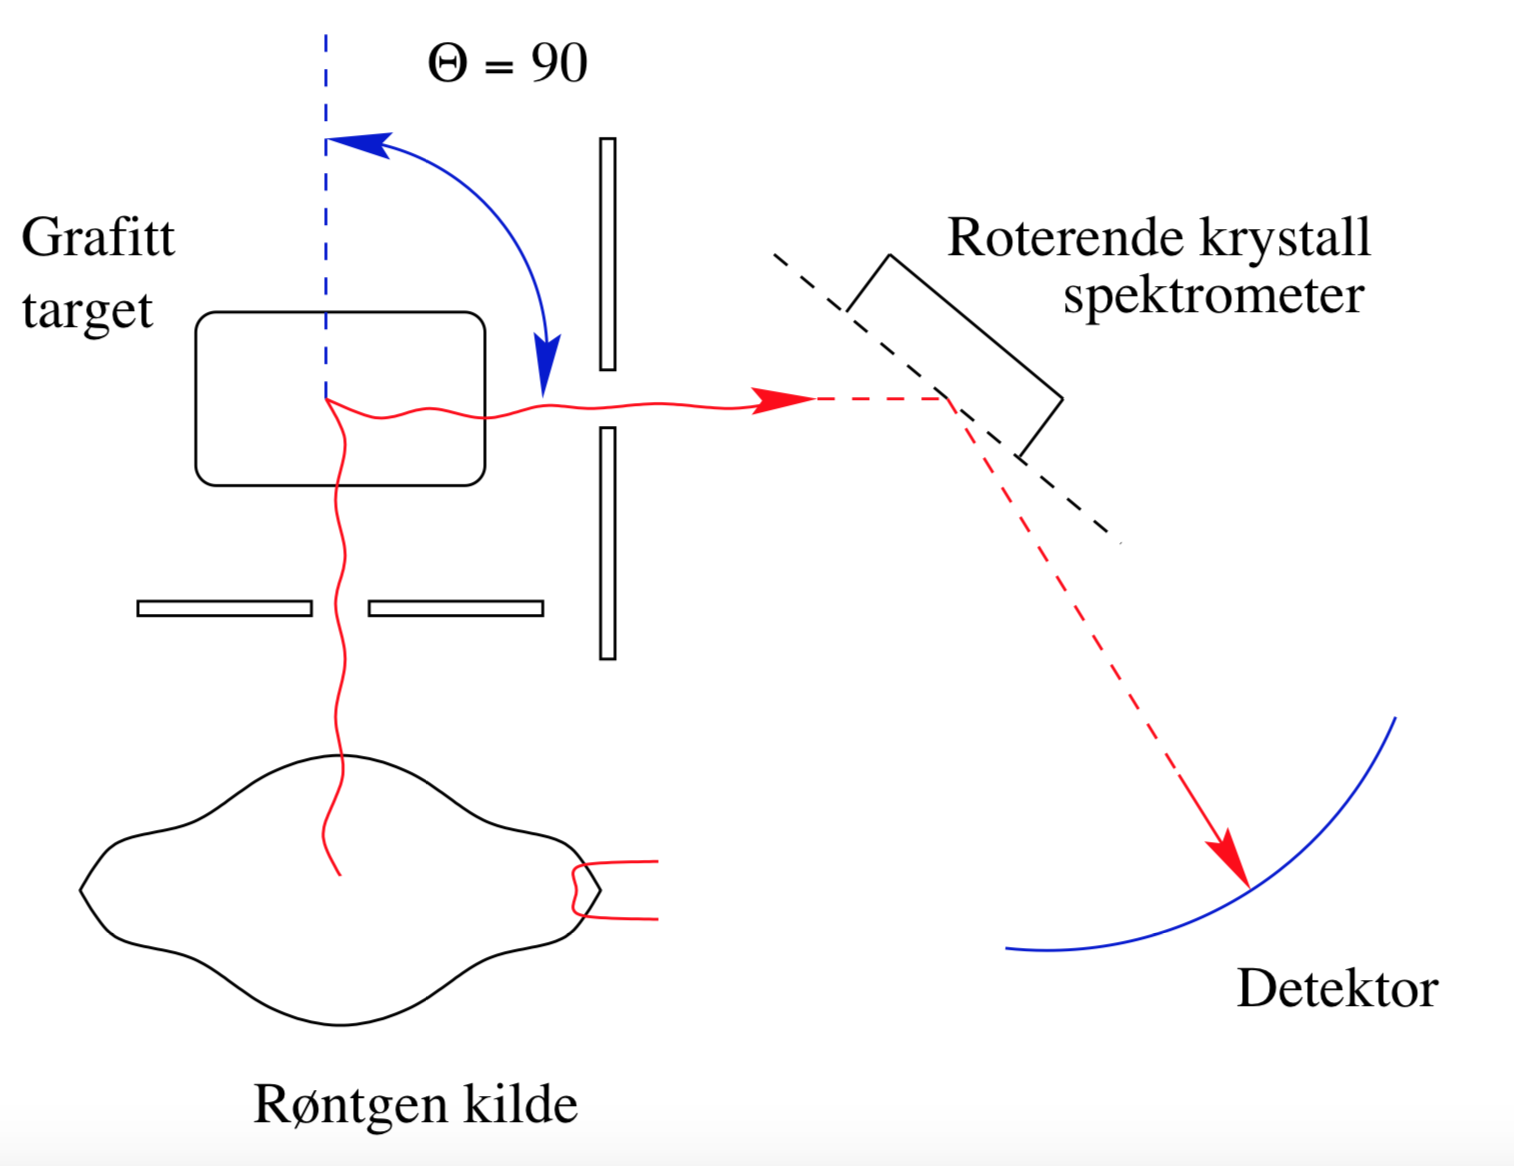
\includegraphics[scale=0.4]{compton}
\caption{Eksperimentelt oppsett for Comptons forsøk, med $\Theta =90$ grader. Bilde hentet fra kompendiet}
\label{fig:compton}
\end{figure}

\subsection*{a2)}

For Fra formel \eqref{eq:1} så har vi 

\begin{align*}
\Delta\lambda &= \lambda_C(1-cos\theta)\\
\end{align*}

Med verdier

\begin{align*}
\lambda &= 0.0709 nm\\
\lambda' &= 0.0749 nm\\
\Delta\lambda &= 0.004 nm
\end{align*}

da får vi

\begin{align*}
\Delta\lambda &= \lambda_C(1-cos\theta)\\
\frac{\Delta\lambda}{\lambda_C} &=  1- \cos \theta\\
\theta &= \cos^{-1}(1- \frac{\Delta\lambda}{\lambda_C})\\
\theta &= \cos^{-1}(1- \frac{0.004nm}{2.43x10^{-3}nm})\\
\theta &= \underline{\underline{130.5^\circ}}
\end{align*}

\subsection*{a3)}


\begin{figure}[h]
\includegraphics[scale=0.4]{intensitetcompton}
\caption{Plot over intensiteten til stråling i Comptons forsøk. $\lambda_0$ er den innkommende strålingen, $\lambda'$ er den spredte strålingen.}
\label{fig:intensitetcompton}
\end{figure}

Toppen i det første plottet i figur \ref{fig:intensitetcompton} og  til venstre i alle de andre plotene i firgur \ref{fig:intensitetcompton}  skyldes forskjell i kollisjon. Når vi har en endring i bølgelengde så vekselvirker fotonet med de elektronene som er svakest bundet til atomet, da gjør vi som fysikerer gjør best og forenkler litt og ser på det som et foton mot et fritt elektron. Men hvis vi tenker at elektroner er sterkt bundet eller at fotonet ikke har nok energi så vil ikke elektronet bli slått løst, dermed blir kollisjonen som en kollisjon mellom et foton og hele atomet. Hvis vi antar at materialet består av karbon så må vi bytte ut massen til elektronet i kollisjonen med massen til et karbonatom. Massen til et karbonatom er ca $22000m_e$. Da blir comptonbølgelengden 

\begin{equation}
\lambda_C = \frac{h}{22000m_ec} \approx 10^{-7} nm = 0.1fm
\end{equation}

Den relative endringen $\frac{\lambda_C}{\lambda}$ blir såvidt observerbar. 
\\

Grunnen til av vi ikke bruker synlig lys til comptoneksperimentet er at synlig lys ikke har nok energi. Synlig lys har nok energi til å kunne få til fotoelektrisk effekt, men ikke til comptonspredning.


\subsection*{b1)}

Vi setter inn verdiene i formelen, $T=25^\circ C = 298.15K$

\begin{align*}
\langle E \rangle &= k_BT\\
\langle E \rangle &= \frac{3}{2} \cdot 8.61 \cdot 10^{-5}  eVK^{-1} \cdot 298.15 K\\
&= 0.0385 \approx \underline{\underline{ 38.5 \cdot10^{-3} eV}}
\end{align*}


\begin{align*}
\langle p \rangle &= \frac{\langle E \rangle}{c} =  38.5 \cdot 10^{-3} eV/c
\end{align*}











\end{document}